\ffigbox[\FBwidth]{%
\caption{\centering Graphe cubique utilisé pour construire \(G_2\)}\label{Fig:exam_blanc_ex_2_2}
}{
    \fbox{
        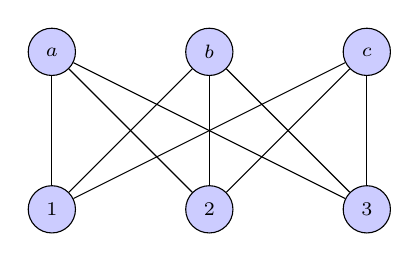
\begin{tikzpicture}[scale=1, main node/.style={circle, draw, fill=blue!20, inner sep=1pt, font=\scriptsize, minimum size=6mm}]
            % graphe biparti 3 3 de taille 6
            \node[main node] (a) at (0,2) {\(a\)};
            \node[main node] (b) at (2,2) {\(b\)};
            \node[main node] (c) at (4, 2) {\(c\)};

            \node[main node] (1) at (0,0) {\(1\)};
            \node[main node] (2) at (2,0) {\(2\)};
            \node[main node] (3) at (4,0) {\(3\)};
            
            % on relie chaque sommet en haut à tous ceux en bas
            \draw (a) -- (1);
            \draw (a) -- (2);
            \draw (a) -- (3);

            \draw (b) -- (1);
            \draw (b) -- (2);
            \draw (b) -- (3);

            \draw (c) -- (1);
            \draw (c) -- (2);
            \draw (c) -- (3);

        \end{tikzpicture}
    }
}